% !TeX root = main.tex

\section{Targeted Inference with Nuisance Parameters}
\label{sec:nuisance}

We extend the sequential contrastive estimation framework to handle nuisance parameters—parameters that must be modeled but are not the focus of inference.
Since $p(h_K|\theta_T,\pi)$ is intractable, we estimate the two required marginals by Monte Carlo:
\begin{itemize}
    \item \textbf{Target marginal}: $M$ samples $\tilde{\theta}_N^{(1:M)} \sim p(\theta_N|\theta_T^{(0)})$ to estimate $p(h_K|\theta_T^{(0)},\pi)$
    \item \textbf{Full marginal}: $L$ contrastive samples $\theta^{(1)},\ldots,\theta^{(L)} \sim p(\theta)$ to estimate $p(h_K|\pi)$
\end{itemize}
Define
\begin{align}
\widehat p_M(h_K|\theta_T^{(0)},\pi)
&:= \frac{1}{M}\sum_{m=1}^{M} p(h_K|\theta_T^{(0)}, \tilde{\theta}_N^{(m)}, \pi), \\
\widehat p_L(h_K|\pi)
&:= \frac{1}{L+1}\sum_{\ell=0}^{L} p(h_K|\theta^{(\ell)}, \pi).
\end{align}

\begin{theorem}[Targeted sPCE Lower Bound]
\label{thm:targeted_spce}
Let $\theta^{(0)} = (\theta_T^{(0)}, \theta_N^{(0)}) \sim p(\theta)$ generate $h_K \sim p(h_K|\theta^{(0)}, \pi)$. Let $\theta^{(1)},\ldots,\theta^{(L)} \sim p(\theta)$ be independent contrastive samples, and let $\tilde{\theta}_N^{(1:M)} \sim p(\theta_N|\theta_T^{(0)})$ be nuisance samples. Define
\begin{equation}
\hat{\mathcal{L}}_K^{\text{tgt}}(\pi, L, M) = \E\left[\log \frac{\widehat p_M(h_K|\theta_T^{(0)},\pi)}{\widehat p_L(h_K|\pi)}\right],
\end{equation}
where the expectation is over $\theta^{(0)}$, the generated history $h_K$, the contrastive samples $\theta^{(1:L)}$, and the nuisance samples $\tilde{\theta}_N^{(1:M)}$.
Assume the relevant likelihoods are positive almost surely so that the logarithms are well defined, and that all displayed expectations are finite.
Then $\hat{\mathcal{L}}_K^{\text{tgt}}(\pi, L, M) \leq \mathcal{I}_K^{\text{tgt}}(\pi)$, with $\hat{\mathcal{L}}_K^{\text{tgt}} \to \mathcal{I}_K^{\text{tgt}}$ as $L, M \to \infty$.
\end{theorem}

\begin{proof}
The gap between the true objective and the practical bound is:
\begin{align}
\mathcal{I}_K^{\text{tgt}} - \hat{\mathcal{L}}_K^{\text{tgt}} &= \E\left[\log \frac{p(h_K|\theta_T^{(0)},\pi)}{p(h_K|\pi)} - \log \frac{\widehat p_M(h_K|\theta_T^{(0)},\pi)}{\widehat p_L(h_K|\pi)}\right] \\
&= \E\left[\log \frac{p(h_K|\theta_T^{(0)},\pi)}{\widehat p_M(h_K|\theta_T^{(0)},\pi)}\right] + \E\left[\log \frac{\widehat p_L(h_K|\pi)}{p(h_K|\pi)}\right].
\end{align}

\textbf{Term 1 (new nuisance-marginalization gap):} Condition on the realized $(\theta_T^{(0)}, h_K)$. Since $\tilde{\theta}_N^{(1:M)} \overset{\text{i.i.d.}}{\sim} p(\theta_N|\theta_T^{(0)})$,
\begin{equation}
\E\big[\widehat p_M(h_K|\theta_T^{(0)},\pi) \mid \theta_T^{(0)}, h_K\big]
= \int p(h_K|\theta_T^{(0)},\theta_N,\pi)\,p(\theta_N|\theta_T^{(0)})\,d\theta_N
= p(h_K|\theta_T^{(0)},\pi).
\end{equation}
Since $\log$ is concave, Jensen's inequality gives
\begin{equation}
\E\big[\log \widehat p_M(h_K|\theta_T^{(0)},\pi) \mid \theta_T^{(0)}, h_K\big]
\leq \log \E\big[\widehat p_M(h_K|\theta_T^{(0)},\pi) \mid \theta_T^{(0)}, h_K\big]
= \log p(h_K|\theta_T^{(0)},\pi),
\end{equation}
and hence
\begin{equation}
\E\left[\left.\log \frac{p(h_K|\theta_T^{(0)},\pi)}{\widehat p_M(h_K|\theta_T^{(0)},\pi)}\,\right|\,\theta_T^{(0)}, h_K\right] \geq 0.
\end{equation}
Taking expectations over $(\theta_T^{(0)}, h_K)$ yields the non-negativity of Term 1.

\textbf{Term 2 (standard sPCE gap):} This term is unchanged by the nuisance extension and is exactly the denominator gap analyzed by \citet{foster2021}. Reusing their change-of-measure and symmetry argument,
\begin{equation}
\E\left[\log \frac{\widehat p_L(h_K|\pi)}{p(h_K|\pi)}\right]
= \E_{p(h_K|\pi)}\left[\text{KL}\left(\tilde{p}(\theta^{(0:L)}|h_K) \,\|\, p(\theta^{(0:L)})\right)\right] \geq 0,
\end{equation}
where $\tilde{p}$ is the same mixture distribution as in the standard sPCE proof. Thus the second term is inherited directly from Foster et al.; the only new ingredient here is Term 1.

Since both terms are non-negative: $\hat{\mathcal{L}}_K^{\text{tgt}} \leq \mathcal{I}_K^{\text{tgt}}$.

\textbf{Convergence:} For the denominator term, we adopt the same bounded likelihood-ratio assumption used by \citet{foster2021}; as they note, it can be weakened, but we keep the simple uniform form here. For the new numerator term, we impose the analogous nuisance-ratio bound. Specifically, assume there exist constants $0<\kappa_{1,N} \le \kappa_{2,N}<\infty$ and $0<\kappa_1 \le \kappa_2<\infty$ such that
\begin{align}
\kappa_{1,N} \le \frac{p(h_K|\theta_T,\theta_N,\pi)}{p(h_K|\theta_T,\pi)} \le \kappa_{2,N} && \forall\,\theta_T,\theta_N,h_K, \\
\kappa_1 \le \frac{p(h_K|\theta,\pi)}{p(h_K|\pi)} \le \kappa_2 && \forall\,\theta,h_K,
\end{align}
Then both log-ratios are uniformly bounded:
\begin{align}
\left|\log \frac{p(h_K|\theta_T^{(0)},\pi)}{\widehat p_M(h_K|\theta_T^{(0)},\pi)}\right|
&\le \max\{ |\log \kappa_{1,N}|, |\log \kappa_{2,N}| \}, \\
\left|\log \frac{\widehat p_L(h_K|\pi)}{p(h_K|\pi)}\right|
&\le \max\{ |\log \kappa_1|, |\log \kappa_2| \}.
\end{align}
By the Strong Law of Large Numbers,
\begin{align}
\widehat p_M(h_K|\theta_T^{(0)},\pi) &\to p(h_K|\theta_T^{(0)},\pi) \quad \text{a.s. as } M\to\infty, \\
\widehat p_L(h_K|\pi) &\to p(h_K|\pi) \quad \text{a.s. as } L\to\infty.
\end{align}
The Bounded Convergence Theorem therefore gives Term 1 $\to 0$ and Term 2 $\to 0$, hence $\hat{\mathcal{L}}_K^{\text{tgt}} \to \mathcal{I}_K^{\text{tgt}}$.
\end{proof}

\section{Computational Budget Trade-offs}
\label{sec:budget_stub}

We briefly summarize how to allocate a fixed simulation budget across the outer minibatch size $B$, the number of contrastive samples $L$, and the number of nuisance samples $M$.
The goal is to approximate the gradient of the targeted expected information gain, $\nabla_\phi\,\mathcal{I}_K^{\text{tgt}}(\pi_\phi)$, as accurately as possible.
Let $\hat g_{B,L,M}(\phi) \in \mathbb{R}^{d_\phi}$ denote the resulting stochastic gradient estimator. For brevity, the bias, variance, and MSE rates below are stated for any fixed gradient coordinate.

\paragraph{Simulation budget (ODE rollouts).}
For mechanistic models, the dominant cost of evaluating $p(h_K|\theta,\pi)$ is simulating the system forward for $K$ design steps.
In our implementation (Algorithm~\ref{algo:DAD}), per episode we perform:
one rollout to generate $h_K$ under $\theta^{(0)}$,
$(L+1)$ rollouts for the denominator likelihoods under $\theta^{(0:L)}$, and
$M$ rollouts for the numerator likelihoods under $(\theta_T^{(0)}, \tilde{\theta}_N^{(m)})$ for $m=1,\ldots,M$.
The nuisance samples require separate ODE solves whenever nuisance parameters enter as initial conditions (e.g., initial biomass $C_{x,0}$) or appear in the dynamics (e.g., $\mu_{\max}$, $K_s$ in Haldane).
Thus, the compute budget is the total number of full-trajectory ODE rollouts per gradient update,
\begin{equation}
\label{eq:budget_rollouts}
\mathcal{C}_{\text{traj}} \;:=\; B\,(L+2+M),
\end{equation}
which is proportional to the number of ODE solver steps per update.

\paragraph{Asymptotic MSE of the gradient estimator.}
Let $g(\phi)=\nabla_\phi\,\mathcal{I}_K^{\text{tgt}}(\pi_\phi)$ denote the true targeted EIG gradient.
Let $\hat g_{B,L,M}(\phi)$ be the stochastic gradient used in training, obtained by differentiating the nested Monte Carlo objective in Theorem~\ref{thm:targeted_spce} and averaging over $B$ simulated episodes.
Under the regularity assumptions needed for the reparameterized gradient estimator and the second-order delta-method expansions used below---namely, interchange of differentiation and expectation, positivity of the Monte Carlo estimators almost surely, and sufficient moment/smoothness control (e.g., finite second and third moments for the relevant likelihood and gradient terms together with finite inverse moments of the Monte Carlo averages near their population means)---as $B,L,M\to\infty$ we have:

\emph{Bias.} At the objective level, Appendix~\ref{sec:nuisance} shows that the numerator term is a Jensen gap and the denominator term is the standard sPCE gap from Foster et al.~\citep{foster2021}. A second-order delta expansion of $\E[\log \widehat p_M\mid \theta_T^{(0)},h_K]$ around $p(h_K|\theta_T^{(0)},\pi)$ gives an $\mathcal{O}(M^{-1})$ numerator bias, while Foster et al. give the corresponding $\mathcal{O}((L+1)^{-1})$ denominator rate. Assuming these objective-level expansions may be differentiated with respect to $\phi$ under the expectation, the gradient bias satisfies:
\begin{equation}
\mathbb{E}[\hat g_{B,L,M}(\phi)] - g(\phi) = \mathcal{O}((L+1)^{-1}) + \mathcal{O}(M^{-1}).
\end{equation}

\emph{Variance.} The estimator averages $B$ independent episodes, so $\mathrm{Var}(\hat g) = \mathrm{Var}(\hat g^{(1)})/B$. The single-episode variance decomposes via the law of total variance into an outer term (from the ground truth and observation noise) and an inner term (from the contrastive and nuisance samples). Conditional on the outer randomness, the numerator contribution depends only on $\tilde{\theta}_N^{(1:M)}$ and the denominator contribution only on $\theta^{(1:L)}$, so their conditional covariance is zero. Moreover, $\nabla_\phi \log \widehat p_M$ is a smooth function of the pair $(\widehat p_M, \nabla_\phi \widehat p_M)$, and similarly for $\nabla_\phi \log \widehat p_L$. A multivariate delta method applied to these pairs gives conditional inner-variance contributions of orders $\mathcal{O}(M^{-1})$ and $\mathcal{O}((L+1)^{-1})$, respectively. Therefore:
\begin{equation}
\mathrm{Var}(\hat g_{B,L,M}(\phi)) = \mathcal{O}(B^{-1}) + \mathcal{O}\big((B(L+1))^{-1}\big) + \mathcal{O}((BM)^{-1}).
\end{equation}

\emph{MSE.} Since $\mathrm{MSE} = \mathrm{Bias}^2 + \mathrm{Var}$ and the cross term in $\mathrm{Bias}^2$ is bounded by the sum of the squared terms (by AM-GM):
\begin{equation}
\label{eq:grad_mse_scaling}
\mathrm{MSE}(\hat g_{B,L,M})
= \mathcal{O}(B^{-1})
+ \mathcal{O}\big((B(L+1))^{-1}\big)
+ \mathcal{O}((BM)^{-1})
+ \mathcal{O}((L+1)^{-2})
+ \mathcal{O}(M^{-2}).
\end{equation}

\paragraph{Optimal scaling under fixed ODE budget.}
Since all three variables $L$, $M$, $B$ consume ODE rollouts, we jointly optimize them under the budget constraint~\eqref{eq:budget_rollouts}.
Substituting $B = \mathcal{C}_{\text{traj}}/(L+2+M)$ into the leading terms of~\eqref{eq:grad_mse_scaling} gives the proxy
\begin{equation}
\mathrm{MSE}(L,M) \;\approx\; \frac{a\,(L+2+M)}{\mathcal{C}_{\text{traj}}} + \frac{c}{(L+1)^2} + \frac{d}{M^2},
\end{equation}
for problem-dependent constants $a,c,d>0$.
This reduction keeps only the leading terms. It is self-consistent: balancing the retained terms yields $L,M \propto \mathcal{C}_{\text{traj}}^{1/3}$ and $B \propto \mathcal{C}_{\text{traj}}^{2/3}$, under which the omitted inner-variance terms $\mathcal{O}((B(L+1))^{-1})$ and $\mathcal{O}((BM)^{-1})$ are both $\mathcal{O}(\mathcal{C}_{\text{traj}}^{-1})$, whereas the retained terms are $\mathcal{O}(\mathcal{C}_{\text{traj}}^{-2/3})$.
Setting $\partial\,\mathrm{MSE}/\partial L = 0$ and $\partial\,\mathrm{MSE}/\partial M = 0$ yields
\begin{equation}
L^\star + 1 = \left(\frac{2c\,\mathcal{C}_{\text{traj}}}{a}\right)^{1/3}, \qquad
M^\star = \left(\frac{2d\,\mathcal{C}_{\text{traj}}}{a}\right)^{1/3}, \qquad
B^\star = \frac{\mathcal{C}_{\text{traj}}}{L^\star + 2 + M^\star}.
\end{equation}
All three scale with $\mathcal{C}_{\text{traj}}$: $L^\star, M^\star \propto \mathcal{C}_{\text{traj}}^{1/3}$ and $B^\star \propto \mathcal{C}_{\text{traj}}^{2/3}$.
Asymptotically, the ratio $(L^\star+1)/M^\star = (c/d)^{1/3}$ depends on the relative magnitudes of the two Jensen gaps.
Equivalently, $B^\star \propto (L^\star+1)^2$ and $B^\star \propto (M^\star)^2$.
When the constants $c,d$ are unknown, a natural default is $c=d$, which gives $L^\star + 1 \approx M^\star$.

\paragraph{Gradient accumulation.}
In practice, GPU memory limits the number of concurrent ODE rollouts.
Gradient accumulation splits the $B$ episodes into $G$ micro-batches of size $B_{\text{micro}} = B/G$ and sums the resulting gradients, so at fixed $L$, $M$, and $B$ it leaves the estimator unchanged. Its role is simply to satisfy the memory constraint
\begin{equation}
(L + M) B_{\text{micro}} \lesssim \texttt{GPU\_MEM}.
\end{equation}
If memory fixes $B_{\text{micro}}$, then increasing $G$ increases the feasible total budget, $\mathcal{C}_{\text{traj}} = G B_{\text{micro}} (L+2+M)$. Re-optimizing $L$, $M$, and $B$ under this larger budget reduces the Jensen-gap bias, at the cost of roughly $G\times$ wall time per update.

\section{Policy Equivalence}
\label{sec:policy_equiv}

We show that the nested adaptive optimization criterion from Section~\ref{sec:criterion} is equivalent to optimizing over policies. Consider $K$ sequential input choices $u_1,\ldots,u_K$ with outcomes $Y_1,\ldots,Y_K$ and utility $U(u_{1:K},Y_{1:K})$. The nested adaptive objective is
\begin{equation}
V = \max_{u_1} \E_{Y_1|u_1}\Big[\max_{u_2} \E_{Y_2|Y_1,u_{1:2}}\Big[\cdots \max_{u_K} \E_{Y_K|Y_{1:K-1},u_{1:K}}[U]\cdots\Big]\Big].
\end{equation}
A deterministic non-anticipative policy $\pi = (\pi_1,\ldots,\pi_K)$ maps histories to inputs: $\pi_1 \in \mathcal{U}_1$ and $\pi_k: \mathcal{H}_{k-1} \to \mathcal{U}_k$ for $k \geq 2$, where $\mathcal{H}_{k-1}$ is the space of histories $(u_1,Y_1,\ldots,u_{k-1},Y_{k-1})$. The policy value is $J(\pi) = \E[U(\pi_1, \pi_2(h_1), \ldots, \pi_K(h_{K-1}), Y_{1:K})]$, with $\Pi$ the set of all such policies.

\begin{theorem}[Policy equivalence]
\label{thm:policy_equiv}
$V = \max_{\pi \in \Pi} J(\pi)$.
\end{theorem}

\begin{proof}
Define continuation values by backward induction:
\begin{align}
G_K(h_{K-1}) &= \max_{a_K \in \mathcal{U}_K} \E[U(u_{1:K-1}, a_K, Y_{1:K}) \mid h_{K-1}, a_K], \\
G_k(h_{k-1}) &= \max_{a_k \in \mathcal{U}_k} \E[G_{k+1}(h_{k-1}, a_k, Y_k) \mid h_{k-1}, a_k],
\end{align}
for $k = K{-}1, \ldots, 1$ (with $h_0 = \varnothing$). By construction, $G_1 = V$.

\emph{Part 1: $\max_\pi J(\pi) \leq V$.}
Fix any $\pi$ and let $V_k^\pi(h_{k-1})$ denote the expected utility under $\pi$ from stage $k$ onward. We show $V_k^\pi(h_{k-1}) \leq G_k(h_{k-1})$ for all $k$ by backward induction.

Base case ($k=K$): $\pi_K(h_{K-1})$ is one feasible action, so
\begin{equation}
V_K^\pi(h_{K-1}) = \E[U \mid h_{K-1}, \pi_K(h_{K-1})] \leq \max_{a_K \in \mathcal{U}_K} \E[U \mid h_{K-1}, a_K] = G_K(h_{K-1}).
\end{equation}
Inductive step: assume $V_{k+1}^\pi(h_k) \leq G_{k+1}(h_k)$ for all $h_k$. Then
\begin{align}
V_k^\pi(h_{k-1}) &= \E[V_{k+1}^\pi(h_k) \mid h_{k-1}, \pi_k(h_{k-1})] \\
&\leq \E[G_{k+1}(h_k) \mid h_{k-1}, \pi_k(h_{k-1})] \\
&\leq \max_{a_k \in \mathcal{U}_k} \E[G_{k+1}(h_k) \mid h_{k-1}, a_k] = G_k(h_{k-1}),
\end{align}
where the first inequality uses the induction hypothesis and the second uses the definition of $G_k$. Setting $k=1$ gives $J(\pi) = V_1^\pi \leq G_1 = V$.

\emph{Part 2: $V \leq \max_\pi J(\pi)$.}
Construct $\pi^\star$ by choosing argmax actions at each stage:
\begin{equation}
\pi_k^\star(h_{k-1}) = \argmax_{a_k \in \mathcal{U}_k} \E[G_{k+1}(h_{k-1},a_k,Y_k) \mid h_{k-1},a_k].
\end{equation}
We show $V_k^{\pi^\star}(h_{k-1}) = G_k(h_{k-1})$ for all $k$ by backward induction.

Base case ($k=K$): $\pi_K^\star$ achieves the argmax, so $V_K^{\pi^\star}(h_{K-1}) = G_K(h_{K-1})$.

Inductive step: assume $V_{k+1}^{\pi^\star}(h_k) = G_{k+1}(h_k)$ for all $h_k$. Then
\begin{align}
V_k^{\pi^\star}(h_{k-1}) &= \E[V_{k+1}^{\pi^\star}(h_k) \mid h_{k-1}, \pi_k^\star(h_{k-1})] \\
&= \E[G_{k+1}(h_k) \mid h_{k-1}, \pi_k^\star(h_{k-1})] \\
&= G_k(h_{k-1}),
\end{align}
where the first equality uses the induction hypothesis and the second uses the definition of $\pi_k^\star$. Setting $k=1$ gives $J(\pi^\star) = V_1^{\pi^\star} = G_1 = V$.
\end{proof}

\section{Bayesian Information Matrix Baseline}
\label{sec:bim}

\paragraph{Static BIM baseline.}
We use a Bayesian D-optimal design criterion based on the Fisher information matrix (FIM) as a baseline. Here $\theta$ denotes only the parameters that enter the dynamics and initial conditions---not the noise parameters. For a static input sequence $u_{1:K}$ and known observation noise covariance $\Sigma$, the FIM is
\begin{equation}
F(\theta, \Sigma, u_{1:K}) = J(\theta, u_{1:K})^\top \Sigma^{-1} J(\theta, u_{1:K}),
\end{equation}
where $J \in \mathbb{R}^{K \times q}$ is the sensitivity matrix with entries $J_{k,j} = \partial g(x(t_k)) / \partial \theta_j$, computed by differentiating the ODE solution. For the Monod bioreactor, $\Sigma = \sigma^2 I$ with $\sigma$ drawn from its prior.

When nuisance parameters are present in $\theta$, we project the information onto the target parameters via the Schur complement. Partitioning the posterior precision $P = F + \Lambda$ (where $\Lambda$ is the prior precision, with $\lambda_j = 12/(\theta_j^{\max} - \theta_j^{\min})^2$ for independent uniform priors) as
\begin{equation}
P = \begin{pmatrix} P_{TT} & P_{TN} \\ P_{NT} & P_{NN} \end{pmatrix},
\end{equation}
the marginal posterior precision for $\theta_T$ is
\begin{equation}
P_T = P_{TT} - P_{TN} P_{NN}^{-1} P_{NT}.
\end{equation}

The Bayesian D-optimal design maximizes the expected log-determinant:
\begin{equation}
u^\star_{\text{BIM}} = \argmax_{u_{1:K}} \; \E_{p(\theta, \Sigma)}\!\left[\log\det P_T(\theta, \Sigma, u_{1:K})\right],
\end{equation}
where the expectation averages over both the dynamics parameters and the noise covariance, approximated by prior samples. This is a standard criterion~\citep{chaloner1995} that assumes Gaussian posteriors (via the Laplace approximation) and does not account for sequential adaptation.
This formulation requires $\Sigma$ to be independent of $\theta$, which precludes our BIM implementation for the pharmacokinetic example, where the noise scales are nuisance parameters that interact with the dynamics parameters in the targeted sPCE objective.
We use the static BIM as a baseline for the Monod bioreactor (Table~\ref{tab:spce}) and the adaptive variant below for the DC motor (Table~\ref{tab:motor}).

\paragraph{Adaptive BIM baseline.}
The adaptive BIM strategy in Table~\ref{tab:motor} extends the static BIM criterion to a sequential, myopic setting. At step~$k$, given the history $(u_{1:k-1}, y_{1:k-1})$:
\begin{enumerate}
\item Compute a MAP estimate $\hat{\theta}_k = \argmax_\theta\, p(\theta \mid y_{1:k-1}, u_{1:k-1})$ via Adam optimization with ForwardDiff gradients (100 iterations, warm-started from $\hat{\theta}_{k-1}$; at $k=1$, initialized at prior midpoints).
\item Select $u_k = \argmax_{u} \log\det P_T(\hat{\theta}_k, [u_{1:k-1}, u])$ by grid search over 100 candidate voltages in $[0, 10]\,$V.
\item Execute $u_k$ on the true system and observe $y_k$.
\end{enumerate}
This replaces the prior expectation $\E_{p(\theta)}[\cdot]$ with a point evaluation at $\hat{\theta}_k$ (a Dirac delta approximation consistent with the Laplace assumption that BIM already makes). The MAP estimate is the natural choice: under the Laplace approximation, MAP coincides with the posterior mean. The strategy is myopic, optimizing one step ahead only.

The key computational difference is that adaptive BIM requires online posterior inference (MAP) and design re-optimization at \emph{each} experimental step, whereas the amortized sPCE policy requires only a single neural network forward pass. This makes adaptive BIM infeasible for real-time applications like the DC motor ($\Delta t = 10\,$ms), where the MAP + grid search takes milliseconds per step and exceeds the sampling interval by the later steps.

\section{Training and Evaluation Details}
\label{sec:training_details}

Training is implemented in Julia~\citep{bezanson2017julia} using Lux.jl~\citep{pal2023lux} for the neural network, Enzyme~\citep{moses2020enzyme} for automatic differentiation through the ODE solver, and Reactant~\citep{reactant2025} for GPU-accelerated compilation via MLIR/XLA. Training was performed on the VSC (Flemish Supercomputer Center) using NVIDIA H100 GPUs.

\paragraph{Architecture.}
The main examples share the same transformer architecture. Each design--observation pair $(u_k, y_k)$ is projected from $\mathbb{R}^2$ to $\mathbb{R}^{32}$ by a dense layer, then summed with 32-dimensional sinusoidal positional encodings. The transformer block consists of RMSNorm, causal multi-head attention (4~heads, dimension~32), and a feed-forward network ($32 \to 64$, GELU, $64 \to 32$). The output head is a dense layer $32 \to 1$ projecting the final hidden state to the design input, with a per-example initial bias (Table~\ref{tab:training_config}). Since the output is passed through a sigmoid, a negative bias initializes the untrained policy to produce small actions, which is more conservative for slow systems like bioreactors.

\paragraph{Optimizer.}
All examples use Adam with a cosine learning rate schedule: linear warmup from $10^{-5}$ to $3 \times 10^{-3}$ over 50~iterations, then cosine annealing back to $10^{-5}$.

\paragraph{Budget allocation.}
For each example, $L$, $M$, gradient accumulation $G$, and micro-batch size $B_{\text{micro}}$ were chosen using the heuristic in Appendix~\ref{sec:budget_stub}, subject to practical memory constraints. Gradient accumulation over $G$ micro-batches yields an effective batch size $B = G \times B_{\text{micro}}$. Table~\ref{tab:training_config} reports the settings used in the reported runs.

\paragraph{ODE integration.}
The dynamics are integrated with a fixed-step RK4 solver, using $N_{\text{sub}}$ substeps per design interval to ensure numerical stability.

A representative training loss curve is shown in Figure~\ref{fig:training_loss}.

\begin{table}[t]
\centering
\caption{Per-example training settings used in the reported runs. The main examples share the architecture and optimizer described above.}
\label{tab:training_config}
\small
\begin{tabular}{@{}lcccc@{}}
\hline
 & Monod & Haldane & Weibull & Motor \\
\hline
Iterations           & 1000 & 1000  & 1000  & 1000 \\
$\mathcal{C}_{\text{traj}}$ & 6.25M & 2.12M & 24M & 56M \\
$G$ (accum.\ steps)  & 8    & 16    & 8     & 8 \\
$L$ (contrastive)    & 464  & 161   & 725   & 960 \\
$M$ (nuisance)       & 466  & 162   & 727   & 962 \\
$B_{\text{micro}}$   & 6706 & 408   & 16506 & 29106 \\
$N_{\text{sub}}$ (RK4) & 50 & 50    & 10    & 10 \\
Output bias          & $-4.0$ & $-1.0$ & $-2.0$ & $0.0$ \\
\hline
\end{tabular}
\end{table}

\begin{figure}[t]
\centering
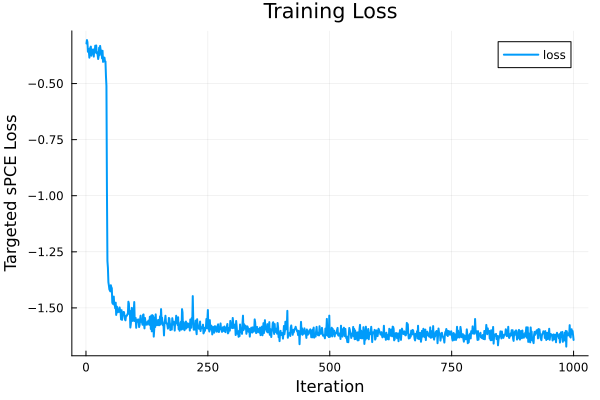
\includegraphics[width=0.7\columnwidth]{figures/monod_training_loss.png}
\caption{Training loss curve (targeted sPCE objective) over iterations for the Monod bioreactor. The objective converges within approximately 1000 iterations.}
\label{fig:training_loss}
\end{figure}

\section{Architecture Ablation}
\label{sec:ablation}

We ablate the transformer-based policy on the Weibull PK model (Section~V) to isolate the contributions of attention and positional encoding. Three architectures are compared, all trained for 200 iterations with the same training setup:
\begin{itemize}
\item \textbf{Full Transformer}: the proposed architecture (attention + sinusoidal PE).
\item \textbf{Flat MLP}: a feedforward network that concatenates the full observation history into a single vector ($48 \to 64 \to 64 \to 1$; 7{,}361 parameters vs.\ 6{,}400 for the transformer).
\item \textbf{Transformer (no PE)}: the same transformer with positional encoding removed.
\end{itemize}

Evaluation uses 1{,}000 paired trials ($L{=}M{=}5{,}000$, $B{=}32$): all three models share the same sampled parameters and noise per trial, so differences are due solely to the architecture. Table~\ref{tab:ablation} reports the results.

\begin{table}[t]
\centering
\caption{Architecture ablation on the Weibull PK model (1{,}000 paired trials, $L{=}M{=}5{,}000$). Higher sPCE is better.}
\label{tab:ablation}
\small
\begin{tabular}{@{}lcc@{}}
\hline
Architecture & sPCE (mean $\pm$ SEM) & Paired $t$ vs.\ Full \\
\hline
Full Transformer      & $1.709 \pm 0.031$ & --- \\
Flat MLP              & $1.679 \pm 0.031$ & $t = 2.24$ ($p < 0.05$) \\
Transformer (no PE)   & $1.364 \pm 0.030$ & $t = 12.09$ ($p < 0.001$) \\
\hline
\end{tabular}
\end{table}

Positional encoding is the dominant factor: without it, the transformer cannot distinguish \emph{when} observations were collected, losing 0.35~nats of expected information. The attention mechanism provides a smaller but statistically significant benefit over the flat MLP (0.03~nats), suggesting that selectively weighting the observation history helps but is less critical than temporal awareness.
